% !TEX root = B99_main.tex

% \begin{figure}
% \begin{center}
% \includegraphics[width=8cm, trim= 0cm 0cm 0cm 0cm,clip]{radiationanalysis.png}
% \caption{Incident radiation on the PV panels. Light blue spots indicate areas of self-shading}
% \label{fig:radiationanalysis}
% \end{center}
% \end{figure}


In this section we show the results of the framework applied to the case study. Section \ref{ch:transient} details the daily performance, this is then expanded in Section \ref{ch:optimal} for results spanning one year. Section \ref{ch:comparison} then compares this performance with a static shading system, and a facade with no shading. For each evaluation the thermal energy demands have been converted to an electrical energy input based on the coefficient of performance of the heating or cooling system.

\subsection{Daily Energetic and Control Profiles of the ASF}
\label{ch:transient}
We run the optimisation for the net energy minimisation. The results, shown in Figure \ref{fig:transient}a detail the simulation run on a sunny day in winter. The dashed line details the optimum altitude angle from an open (90$^{\circ}$), to a closed (0$^{\circ}$) position, and the azimuth angles from a south-east facing (45$^{\circ}$) to a south-west facing (-45$^{\circ}$) direction. We can see that the the azimuth angles start at an east facing position, roughly around 30$^{\circ}$, and switches to a west facing position, around -30$^{\circ}$ in the afternoon. The building energy demand consists of heating (H) and lighting (L) loads in the morning and evening. We can see that between 10:00 to 15:00 the PV panels are capable of generating more electricity (PV) than the office requires. 

Figure \ref{fig:transient}b compares this simulation with a sunny day in summer. The main energetic difference is the presence of a cooling (C) load in the afternoon. The panels still move in the azimuth directions from east to west, however the panels in the altitude direction sit at a higher angle to catch the higher sun position. The patterns in the summer and winter cases are representative of a solar tracking model, however, in both cases it appears to be limited between $\pm$30$^{\circ}$. This is most likely due to high module self-shading at $\pm$45$^{\circ}$, resulting in a large decrease in the PV module efficiency. In winter, the altitude angle is relatively stagnant at 15$^{\circ}$. This angle is sufficient to maximise the PV electricity generation, while still allowing enough solar penetration into the room to keep the lighting and heating demands to a minimum. 

In comparison, Figure \ref{fig:transient}c, details an optimisation on the same winter day, purely to minimise the heating load. In this case, the PV electricity generation, lighting demand, and cooling demand are not taken into account. There are two observable differences in the choice of angles. Firstly, the angles in the altitude position are mostly in the open (90$^{\circ}$) position. Secondly, the azimuth angles follow an inverse solar tracking methodology, starting with west facing angles in the morning, and moving to east facing directions in the evening. Both effects maximise the solar penetration into the room and therefore minimise the heating demand (red line), at the expense of the PV electricity generation (gold line). A similar comparison was conducted for the summer case where a simulation was run purely to optimise the cooling load as seen in \ref{fig:transient}d. The optimum angles to minimise cooling are similar to the optimum angles to minimise net energy so there are only minor differences in the chosen angles.
%However, these minor differences increase the PV generation by 19.5\%, and decreases the lighting by 50\% with only a 5\% increase in the cooling load. This ultimately decreases the net energy consumption of the day from 1151 Wh to 132 Wh.

It is also interesting to note that a sunny day in winter produces 3.0kWh of electricity, while a sunny day in summer produces only slightly more at 3.8kWh in the net energy optimisation case. This is due to the variation in the sun position. The  low winter sun position combined with solar tracking means that the panels are often perpendicular to the direction of the solar radiation. In summer, on the other hand, there is a high sun position, resulting in module self-shading which decreases the efficiency of the PV panels. Over the full day, the PV electricity supply compensates for 62\% of the energy demand on this sunny winters day, and 270\% of the energy demand on a sunny summers day. 


% \begin{figure}
% \begin{center}
% 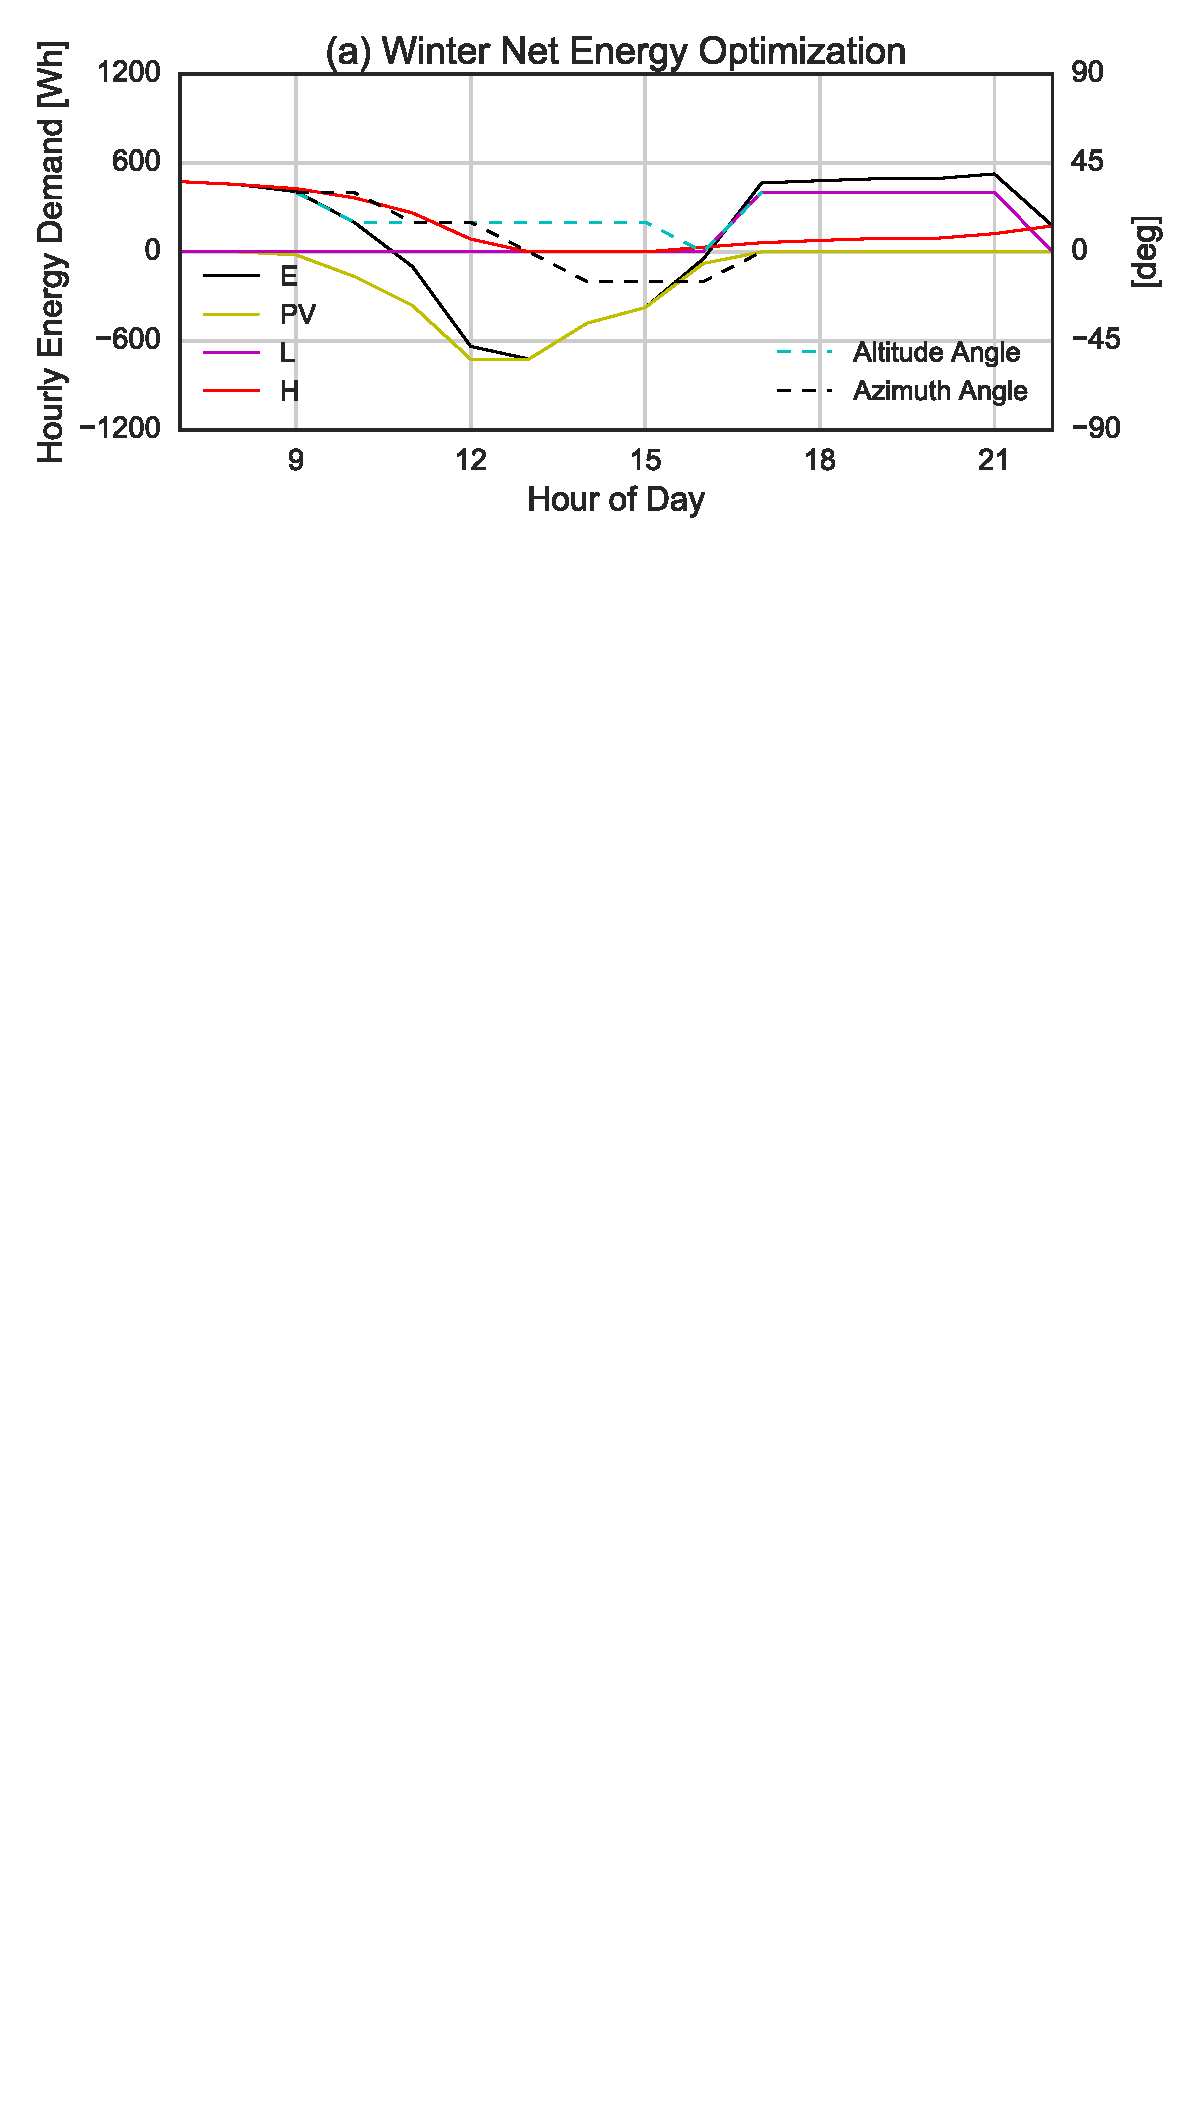
\includegraphics[width=\textwidth, trim= 0cm 0cm 0cm 0cm,clip]{HourlyPlot_WinterNew.pdf}
% \caption{Net energy optimisation and adaptation of the ASF on a sunny day in winter. The solid lines detail the energy balance of heating (H), lighting (L), PV electricity production (PV) and net energy (E) in Watt-hours. The dashed lines detail the panel position in the altitude angle from open (90$^{\circ}$), to a closed (0$^{\circ}$) position, and in the azimuth direction from a south-east facing (45$^{\circ}$) to a south-west facing (-45$^{\circ}$) direction. Only daylight hours are shown for the angle optimisation}
% \label{fig:transientWinter}
% \end{center}
% \end{figure}

\begin{figure}
\begin{center}
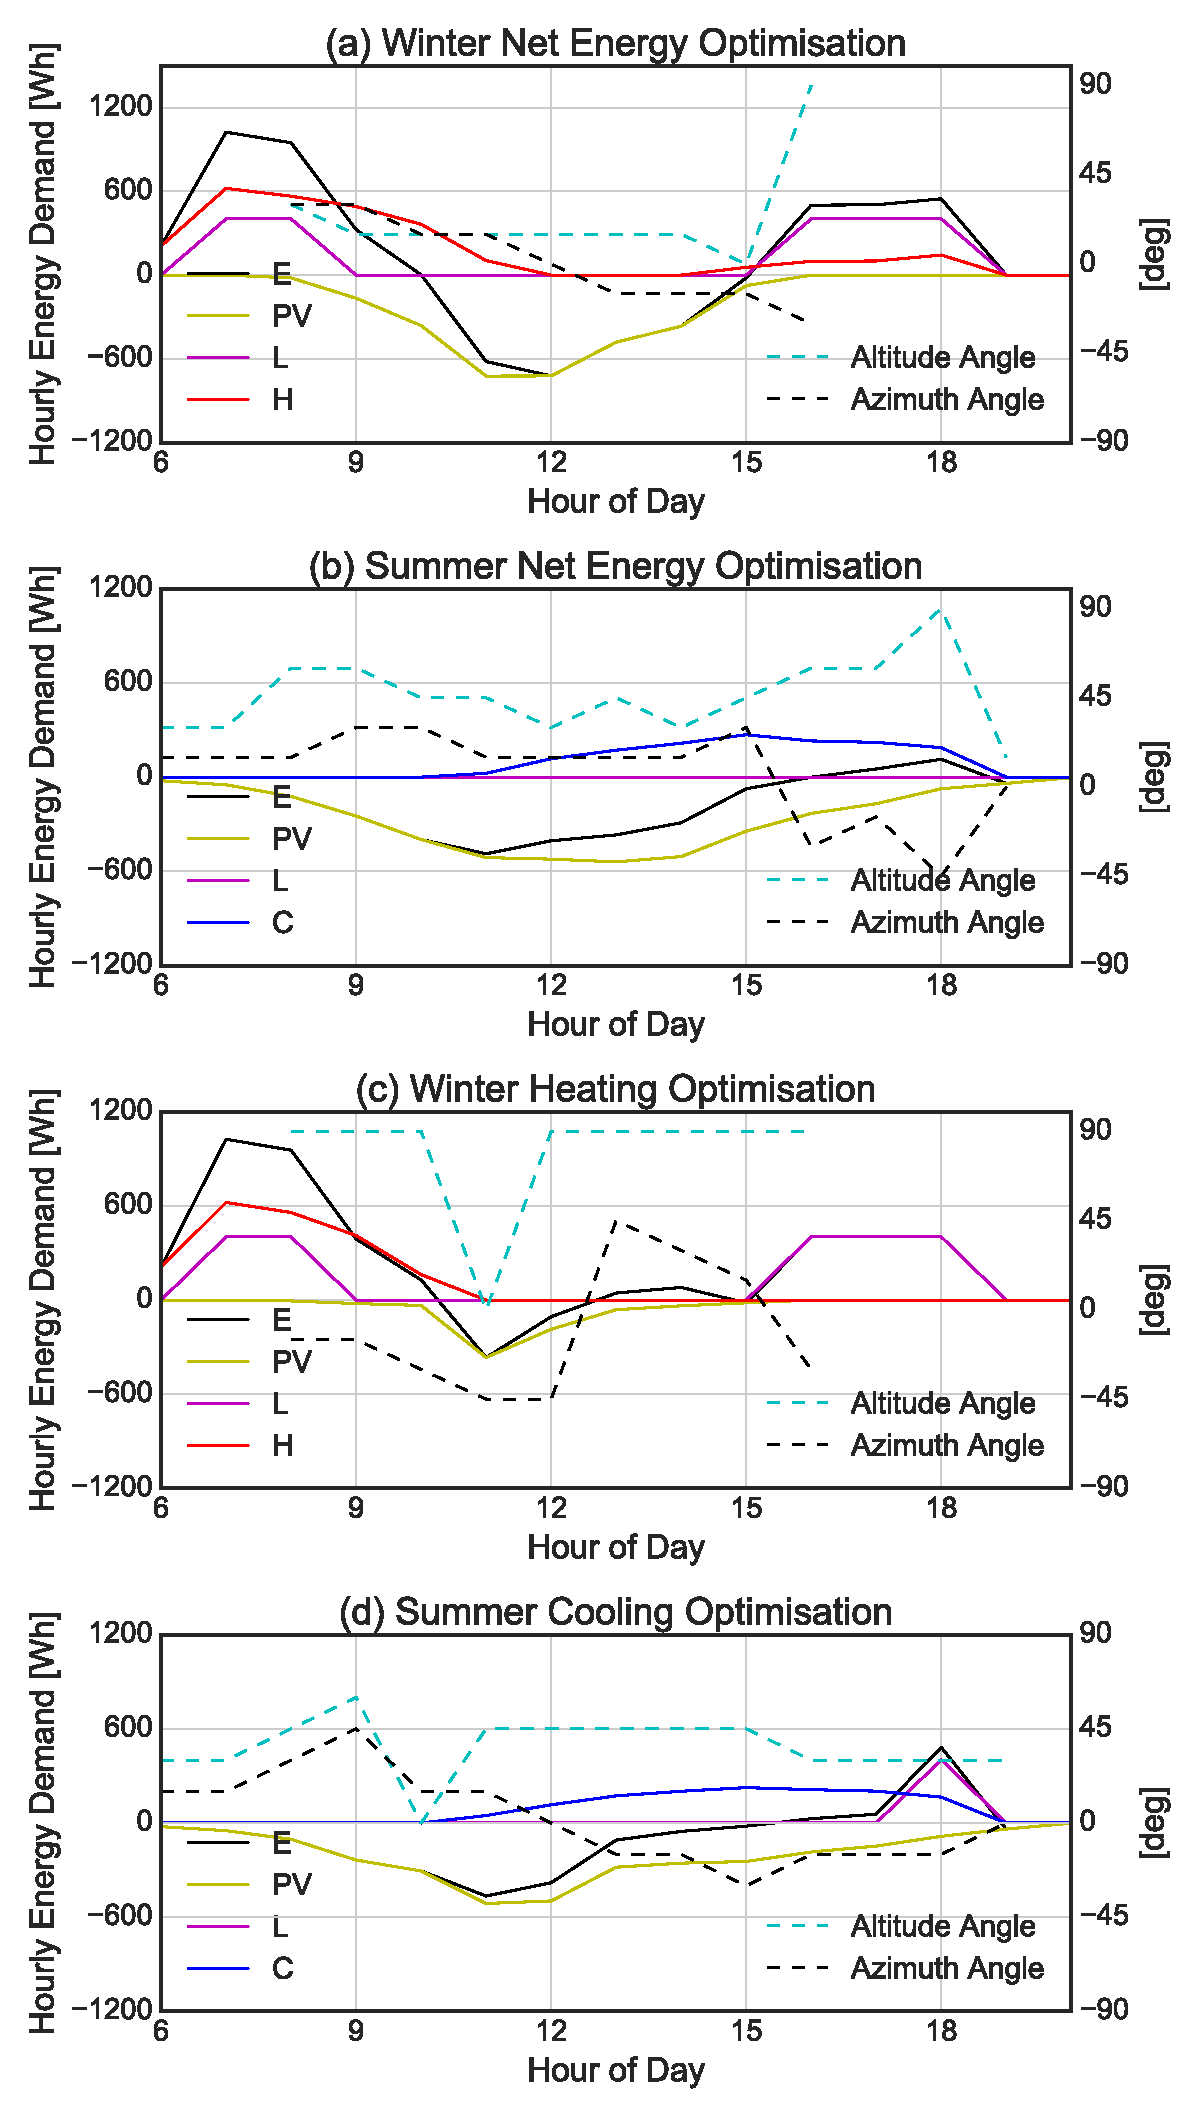
\includegraphics[width=0.65\textwidth,, trim= 0cm 0cm 0cm 0cm,clip]{HourlyPlotNew3.pdf}
\caption{Net energy optimisation and adaptation of the ASF on a sunny day in winter (a) and summer (b). The solid lines detail the energy balance of heating (H), lighting (L), Cooling (C), PV electricity production (PV) and net energy (E) in Watt-hours. The dashed lines detail the panel position in the altitude angle from open (90$^{\circ}$), to a closed (0$^{\circ}$) position, and in the azimuth direction from a south-east facing (45$^{\circ}$) to a south-west facing (-45$^{\circ}$) direction. Only daylight hours are shown for the angle optimisation. In Figures (c) - (d) the optimisation is restricted to just the heating optimisation and cooling optimisation in winter and summer respectively.}
\label{fig:transient}
\end{center}
\end{figure}

\subsection{Optimum Annual Configurations}
\label{ch:optimal}

The optimal configurations of the ASF case study over a year can be visualised using heat-maps. Figure \ref{fig:monthly_altitude} and \ref{fig:monthly_azimuth} detail the optimal angle in the altitude and azimuth angles respectively. To accelerate the radiation analysis, the weather data for each month is averaged to acquire data for a typical day of that month. Figure \ref{fig:monthly_altitude}a-d detail optimisations of individual objectives. We can see how open configurations (light colours) are often chosen for the minimisation of the heating and lighting demands. Likewise, closed configurations (dark colours) are the preferred solutions to minimise the cooling demand during the summer months. Interestingly, this trend appears to inverse during the summer months at midday. The high sun position favours open positions to maximise shading thus minimising cooling in summer. Likewise closed positions with maximum tilt in the azimuth angle maximise solar penetration, and thus minimise heating. The grey coloured points indicate times where there is no sun and therefore the ASF has no influence on the results. 
%Black coloured points areas where there is the combination of the ASF has no impact on the energy load. For example, in summer, no heating is required, therefore there is no optimal angle combination to reduce this any further. 

%The PV optimisation, best seen in Figure \ref{fig:monthly_azimuth}(d), follows a path similar to a classic solar tracking model. The variation from a solar tracking model is due to the effects of self-shading. 

\begin{figure*}
\begin{center}
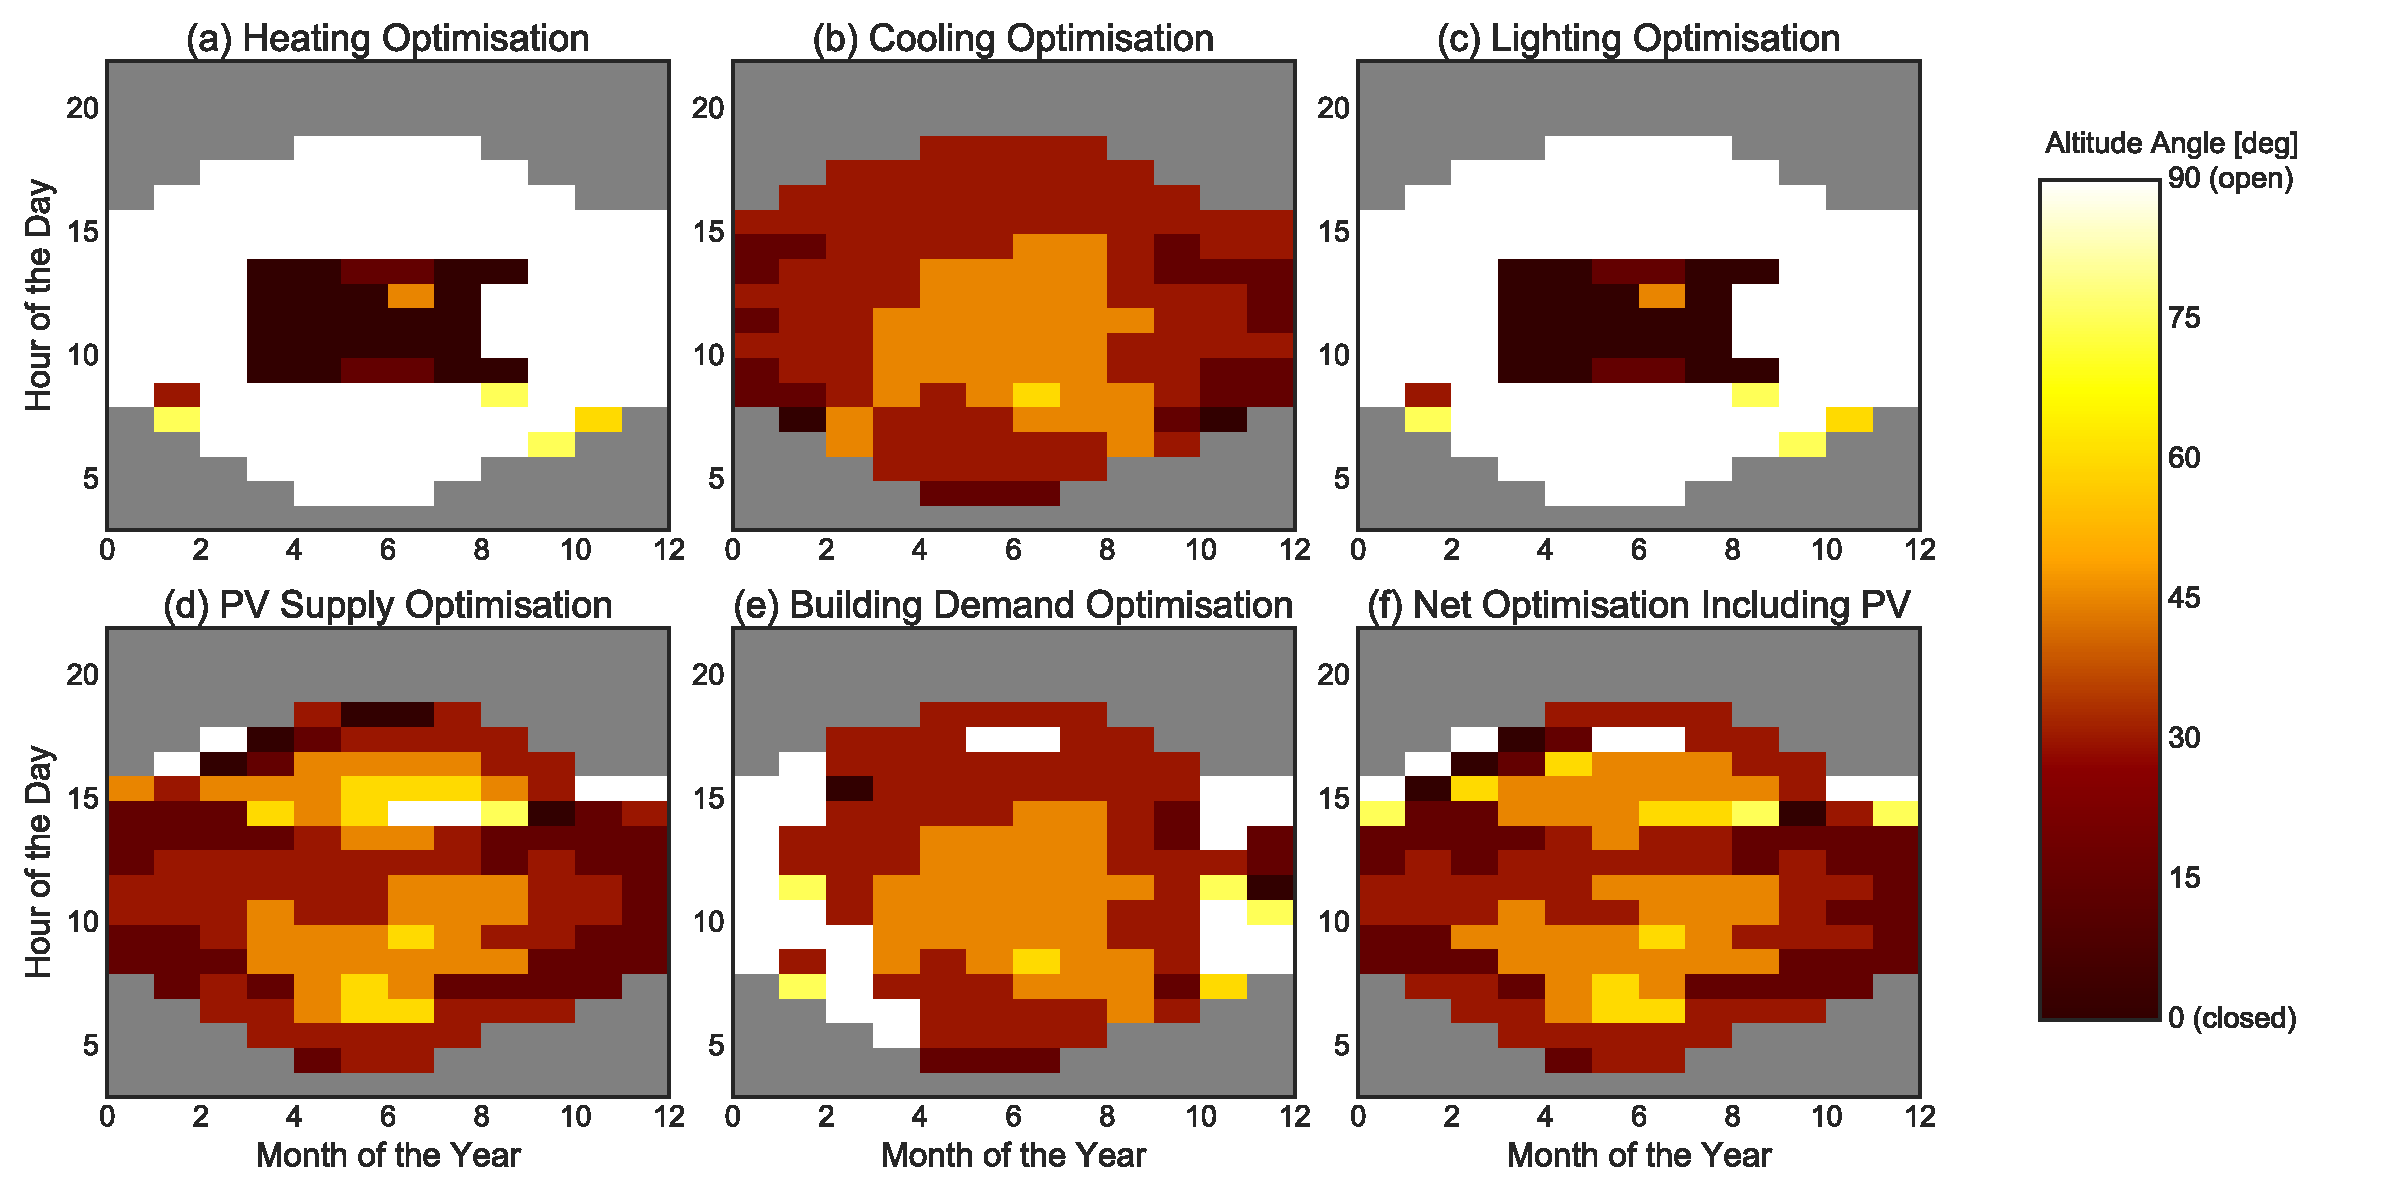
\includegraphics[width=\textwidth, trim= 0cm 0cm 0cm 0cm,clip]{Altitude.pdf}
\caption{Carpet plots detailing the optimal altitude angles to minimise the heating demand(a), cooling demand (b), lighting demand (c), and maximise PV electricity production (d). (e) details the combinations for optimum building thermal management without PV production, (f) also includes the PV production. Small angles correspond to closed positions, whereas large angles represent open positions. The corresponding azimuth angles for each hour are shown in Figure \ref{fig:monthly_azimuth}.}
\label{fig:monthly_altitude}
\end{center}
\end{figure*}

\begin{figure*}
\begin{center}
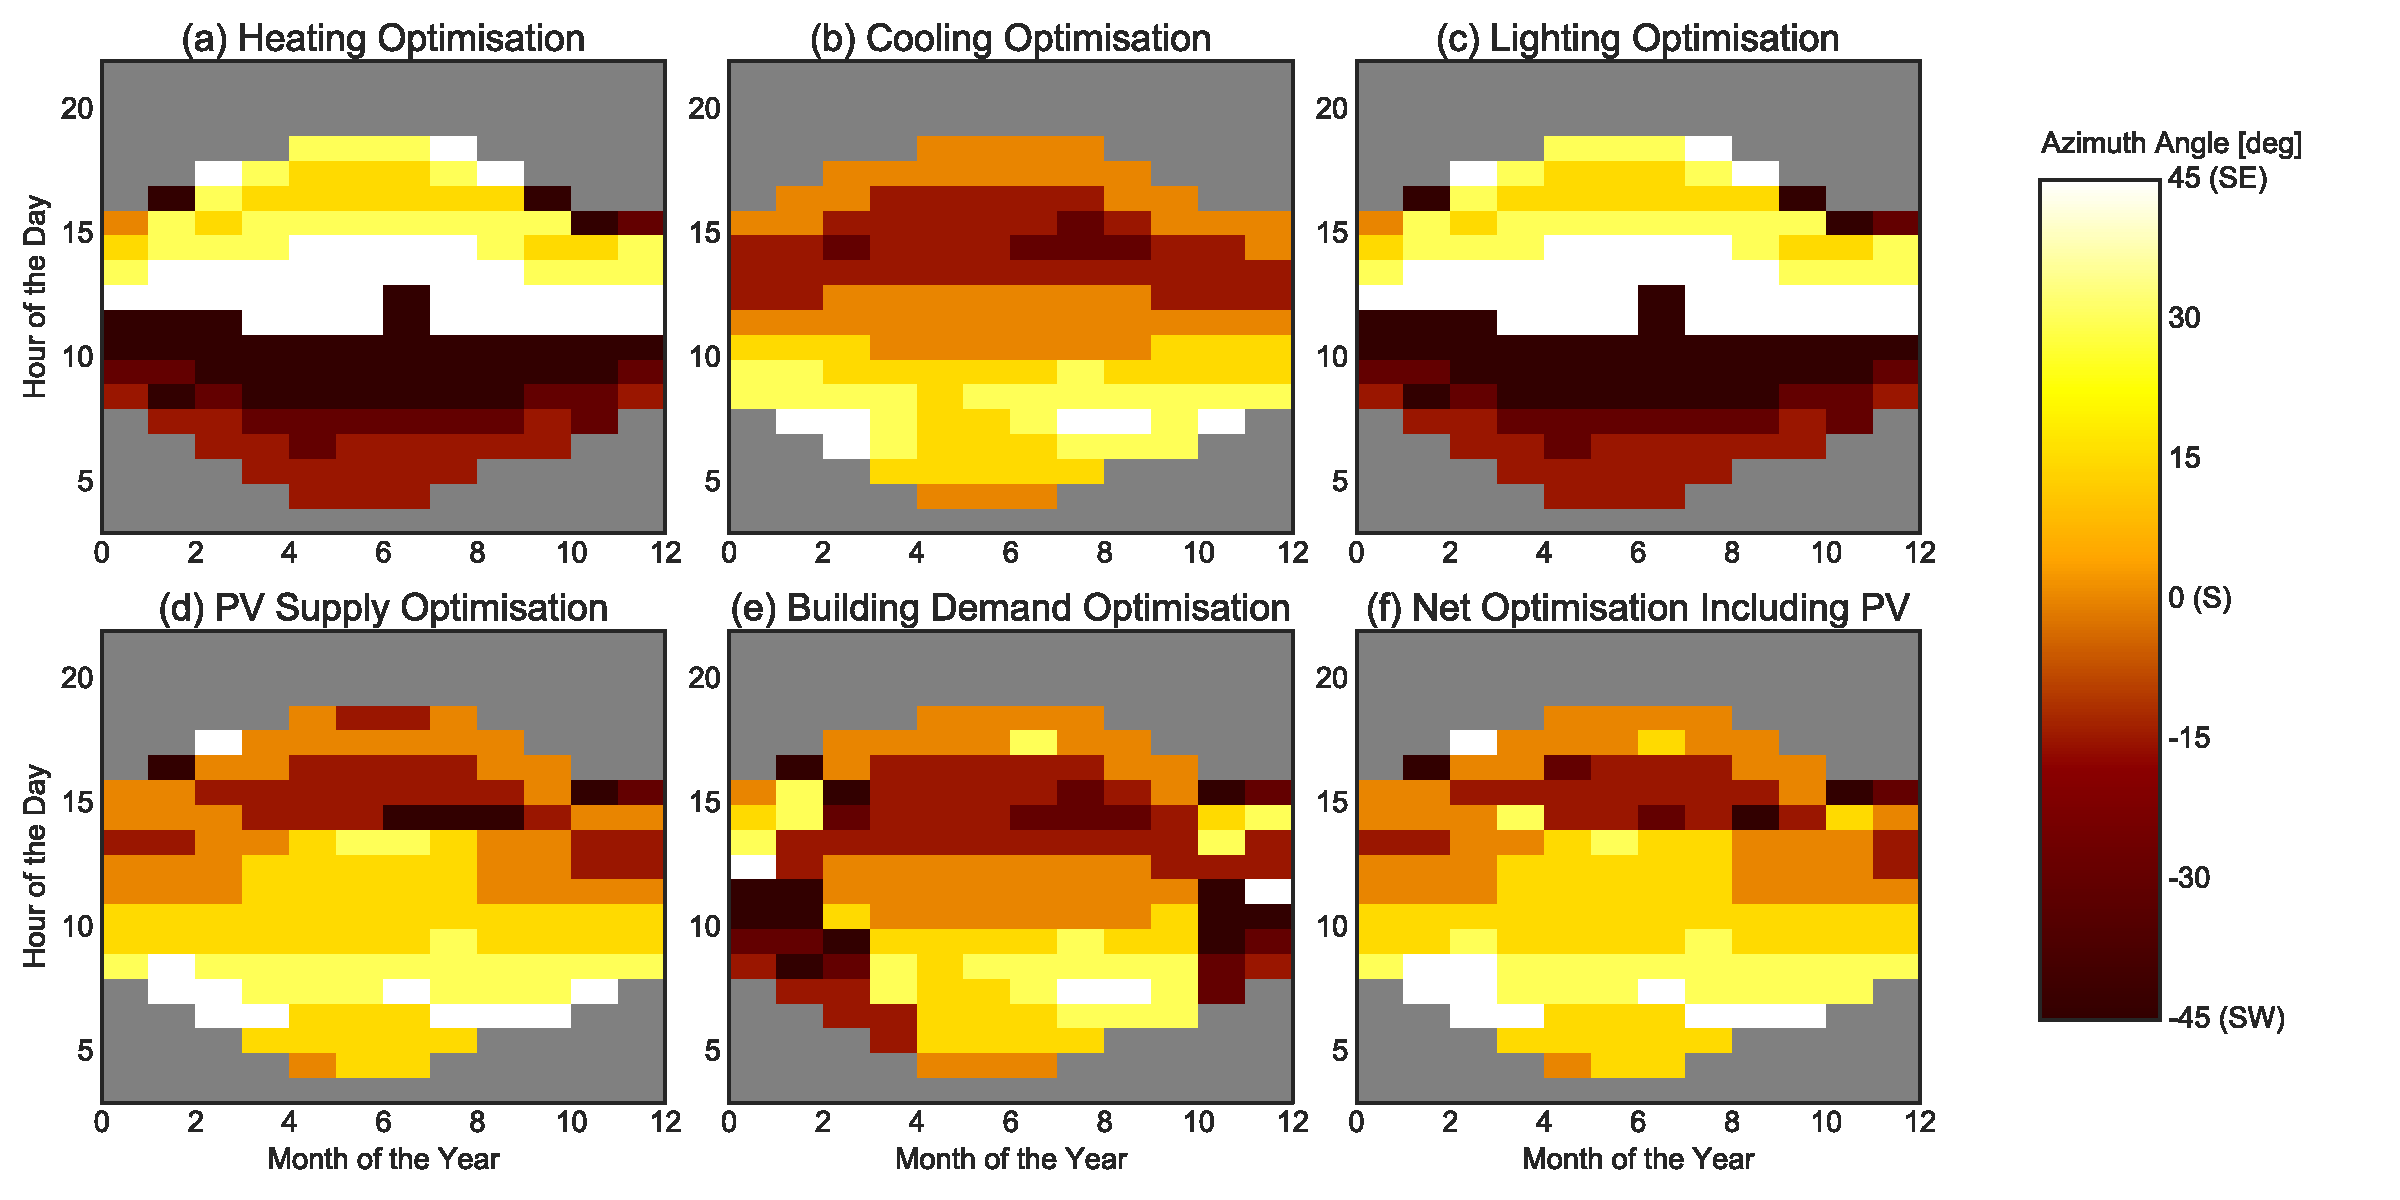
\includegraphics[width=\textwidth, trim= 0cm 0cm 0cm 0cm,clip]{Azimuth.pdf}
\caption{Carpet plots detailing the optimal azimuth angles to minimise the heating demand (a), cooling demand (b), lighting demand (c), and maximise PV electricity production (d). (e) details the combinations for optimum building thermal management without PV production, (f) also includes the PV production. Negative angles correspond to the panels facing west, whereas positive angles represent east-facing panels. The corresponding altitude angles for each hour are shown in Figure \ref{fig:monthly_altitude}.}
\label{fig:monthly_azimuth}
\end{center}
\end{figure*}



%When the four optimisation cases are combined to achieve the configurations for total energy minimisation we get some interesting results seen in Figure \ref{fig:monthly_altitude}(e) and \ref{fig:monthly_azimuth}(e). We can see that during the twilight hours of the morning and evening the open positions are preferred to minimise the use of artificial lighting. During the summer afternoons, closed positions to minimise cooling demands are preferred, however enough light is allowed to pass to sufficiently illuminate the space. When we also include the PV electricty optimisation we notice a strong tendency of the ASF to follow an optimal PV production pattern. This, however changes if the building system becomes more inefficient. Less efficient heating, for example, would result in configurations optimised for heating overpowering those of PV electricity generation.

When the four optimisation cases are combined to achieve the configurations for total energy minimisation we get interesting results, as seen in Figure \ref{fig:monthly_altitude}f and \ref{fig:monthly_azimuth}f. We see a clear tendency of the ASF to follow an optimal PV production pattern with the exception of the mid-winter evenings where heating and lighting are important. This means that it is energetically favourable to heat the room through solar radiation heat gains rather than converting the solar radiation into electricity which is then used for room heating. Configurations to reduce cooling demand are complimentary with the PV supply optimisation and therefore have a minor influence on the system control. 
%Note that these patterns were generated for a specific case study highlighted in Table \ref{tab:AssumptionsOpp}. Having a more inefficient building system may favour configurations to reduce the building energy demand over PV generation.\\


%\subsection{Net Energy Consumption}

Figure \ref{fig:carpetplot_energy} shows the net electricity use. Red colours detail the electrical consumption intensity, and blue colours detail the PV electricity surplus. It is interesting to see in Figure \ref{fig:carpetplot_energy}f how the combination of electricity generation and adaptive shading can compensate for the energy consumption of the building during most sunlit hours. Overall the PV electricity compensates for 61\% of the energy demand of the office behind the facade during the course of the year in the net energy optimisation case.

\begin{figure*}
\begin{center}
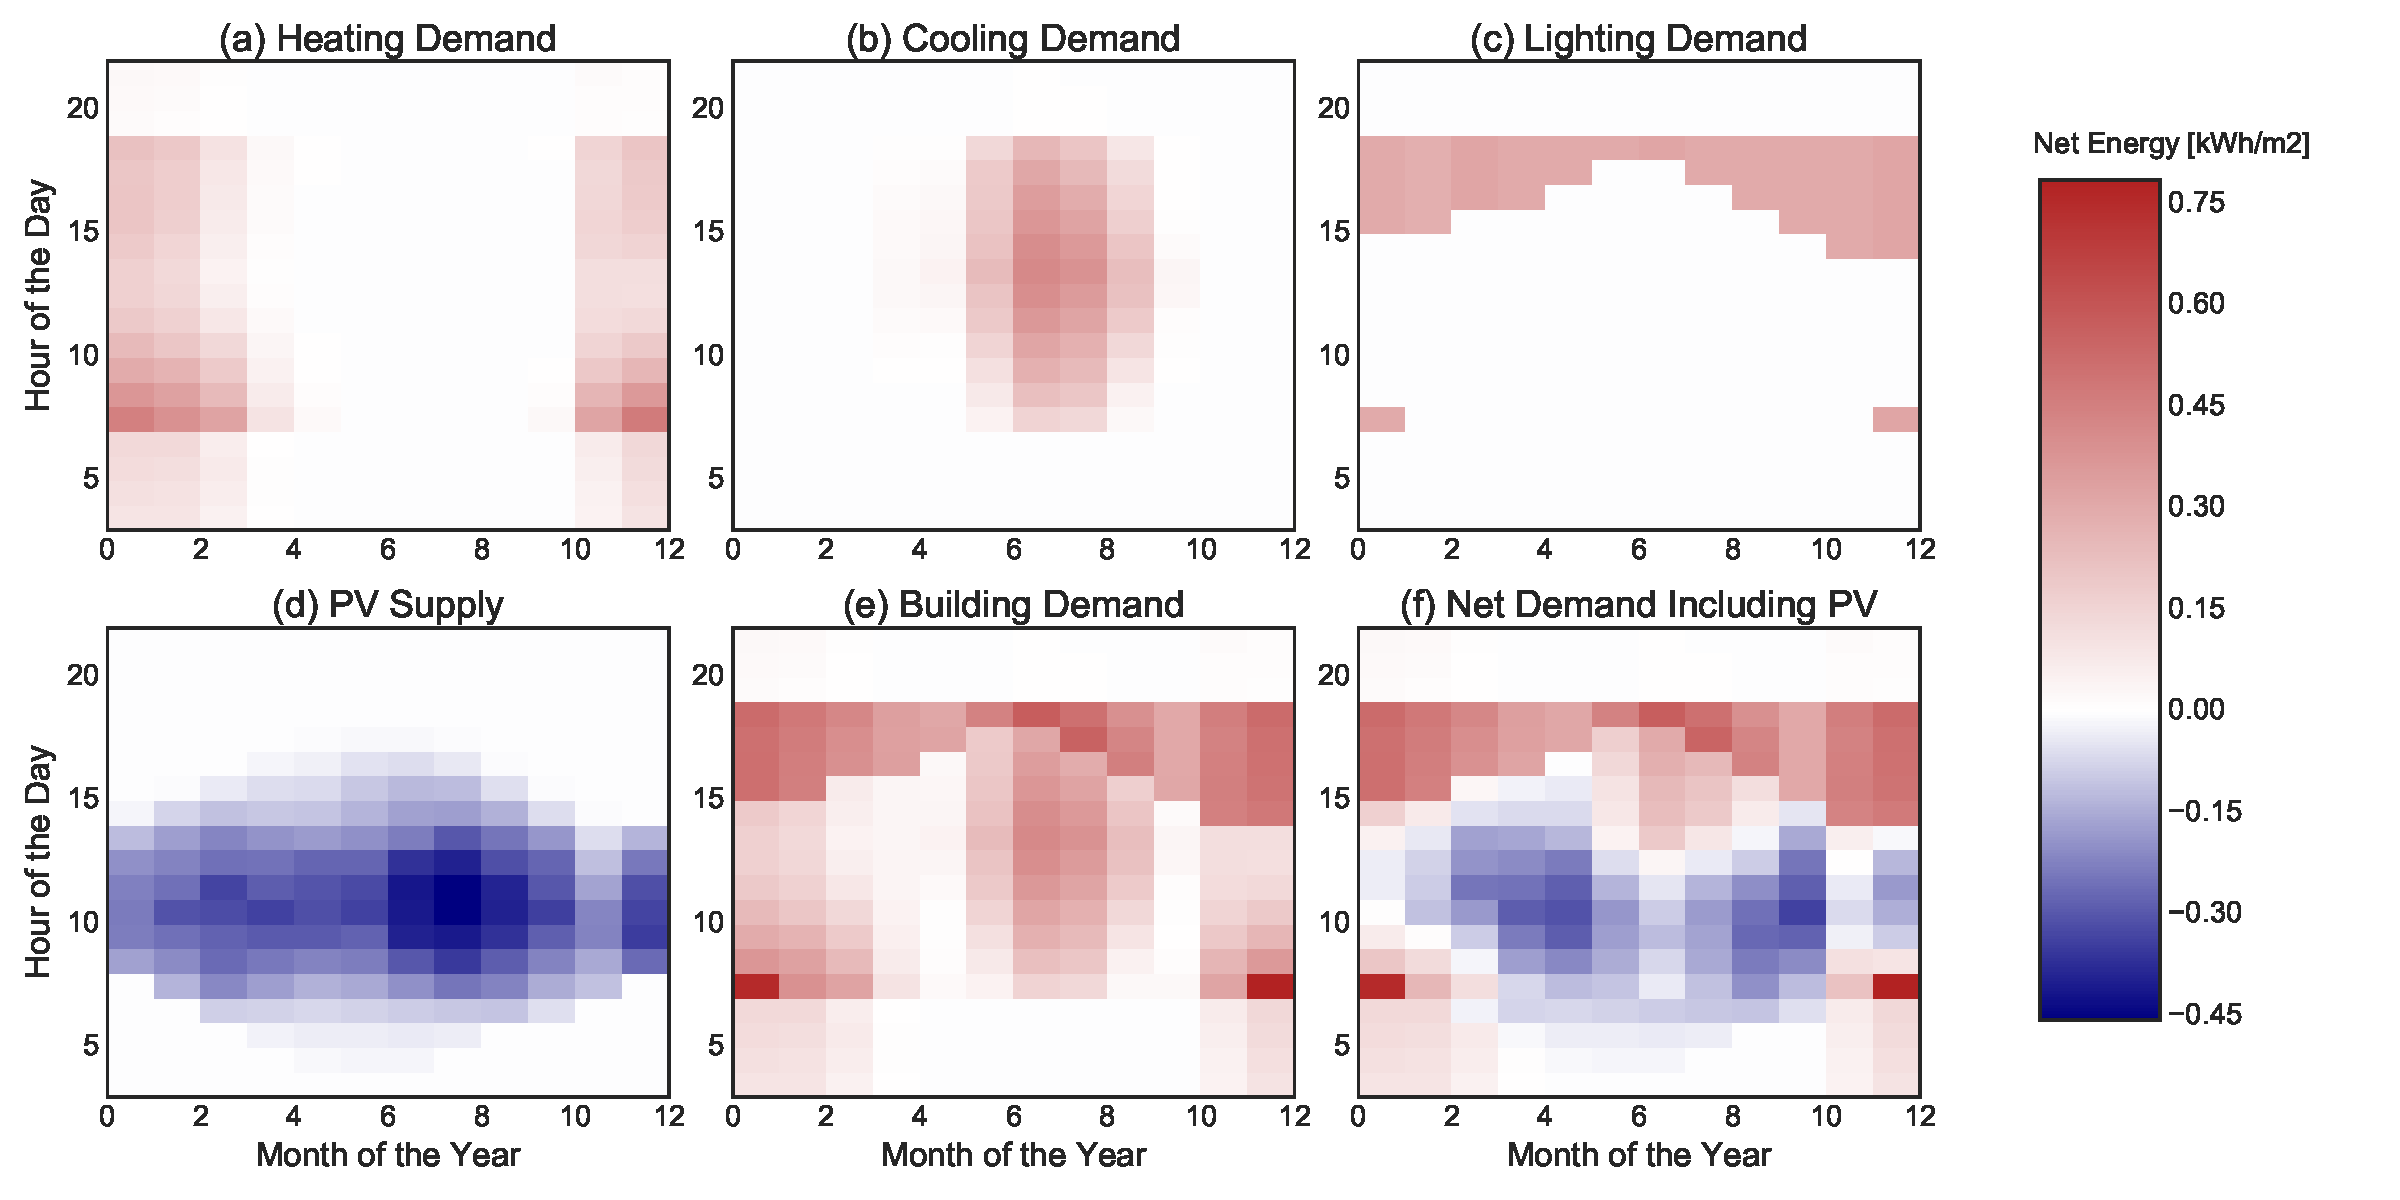
\includegraphics[width=\textwidth, trim= 0cm 0cm 0cm 0cm,clip]{carpetplot_energy3.pdf}
\caption{Carpet plots detailing the net energy consumption. Each square represents the total energy consumption for that specific hour of the entire month. Red colours detail net energy consumption, while blue colours detail net energy production.}
\label{fig:carpetplot_energy}
\end{center}
\end{figure*}


\subsection{Comparison With Other Systems}
\label{ch:comparison}

%\deleted[id=pj2]{Figure \ref{fig:compare} shows the difference between a glazing with no shading system, a static shading system, and an adaptive shading system. A south facing facade with standard glazing and no shading system would always have an overheating issue which can be seen with the large cooling load. Note that in the model there is no restriction of the heating or cooling system. This means that the cooling or heating is assumed to always meet the demand. The optimum orientation of static panels was calculated using the same simulation framework, and an orientation of 45$^{\circ}$ to the horizontal axis is a configuration close to the energy optimal state. By enabling adaptability we see how the heating load can be reduced, without compromising the cooling savings through shading. Overall, the adaptive system has a 20\% savings in the building energy demand, and a 7\% increase in PV electricity production over the static variant. }

Figure \ref{fig:compare} shows the difference between a window with no shading system, a static shading system, and an adaptive shading system which minimised net energy demand, for various coefficients of performance of the heating and cooling system. The optimum orientation of the static shading system was calculated using the same simulation framework, and a panel inclination of 45$^{\circ}$ in the altitude direction is close to the energy optimal state.

Figure \ref{fig:COP11} details an example of an inefficient building system with resistive electrical heating and a low efficiency cooling heat pump. We can see how having a simple static shading system can have a large reduction in the cooling demand with an increase in the heating demand. By including adaptability the same reduction in cooling is possible with a reduced increase in the heating demand. This effect becomes more pronounced in Figure \ref{fig:COP13} where a standard heat pump is added for cooling. Here the comparison between a static shading system and no shading is similar to the results obtained by Palmero-Marrero et al. where the reduction in the cooling demand is offset by the increase in heating demand \cite{palmero2010effect}. An adaptive facade is able to negate this loss resulting in a 44\% net energy saving compared to a building with a static facade. When an efficient heat pump heating system is also included, as detailed in Figure \ref{fig:COP33}, there is an increase in PV electricity supply by 19\%, but a negligible change in the building energy demand. This is because the angles that maximise photovoltaic generation are preferred over angles that reduce the heating demand as there is a larger net energy saving. The same results apply to a highly efficient building case as detailed in Figure \ref{fig:COP66}. Interestingly in this case, the PV supply of the ASF can almost compensate for the entire energy demand of the office space behind it. The results are summarised in Table \ref{tab:compare}.


\begin{figure}
    \centering
    \begin{subfigure}[b]{0.47\textwidth}
        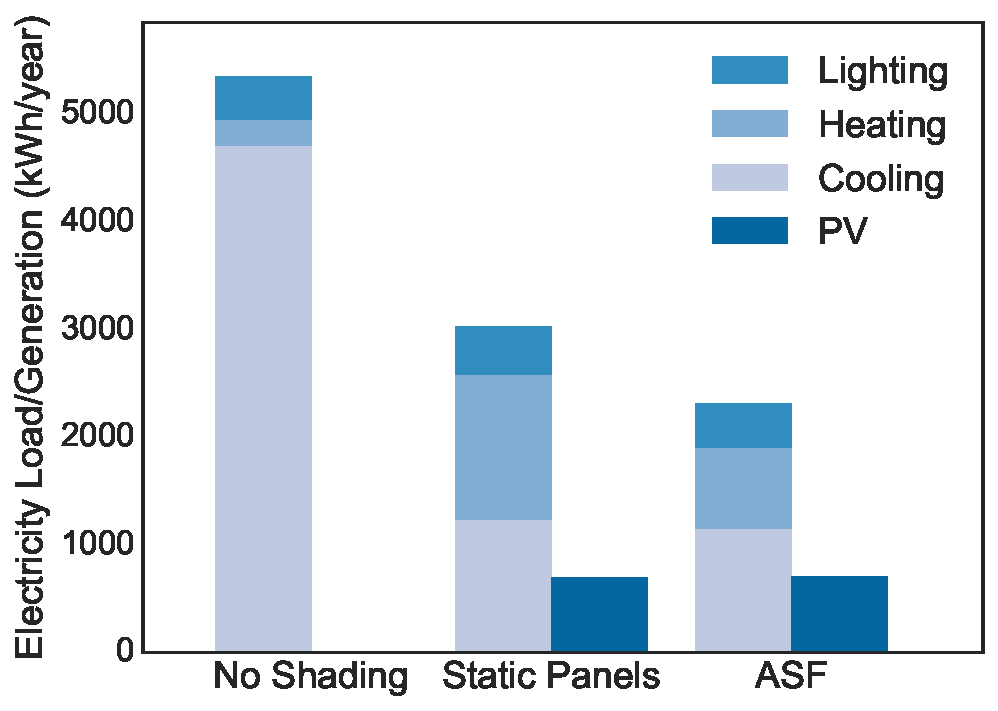
\includegraphics[width=\textwidth]{compare_facadesCOP1.pdf}
        \caption{$COP_{heating}=1$, $COP_{cooling}=1$} 
        \label{fig:COP11}
    \end{subfigure} \hfill
    \begin{subfigure}[b]{0.47\textwidth}
        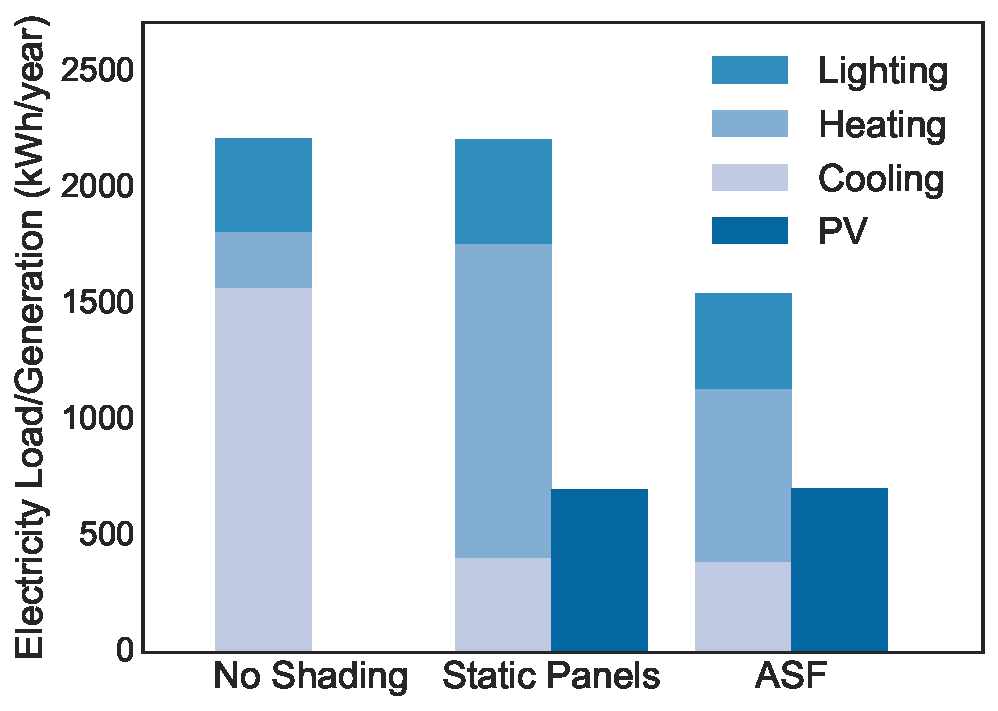
\includegraphics[width=\textwidth]{compare_facadesCOP1_3.pdf}
        \caption{$COP_{heating}=1$, $COP_{cooling}=3$}
        \label{fig:COP13}
    \end{subfigure}
    \vspace{10mm}

    \begin{subfigure}[b]{0.47\textwidth}
        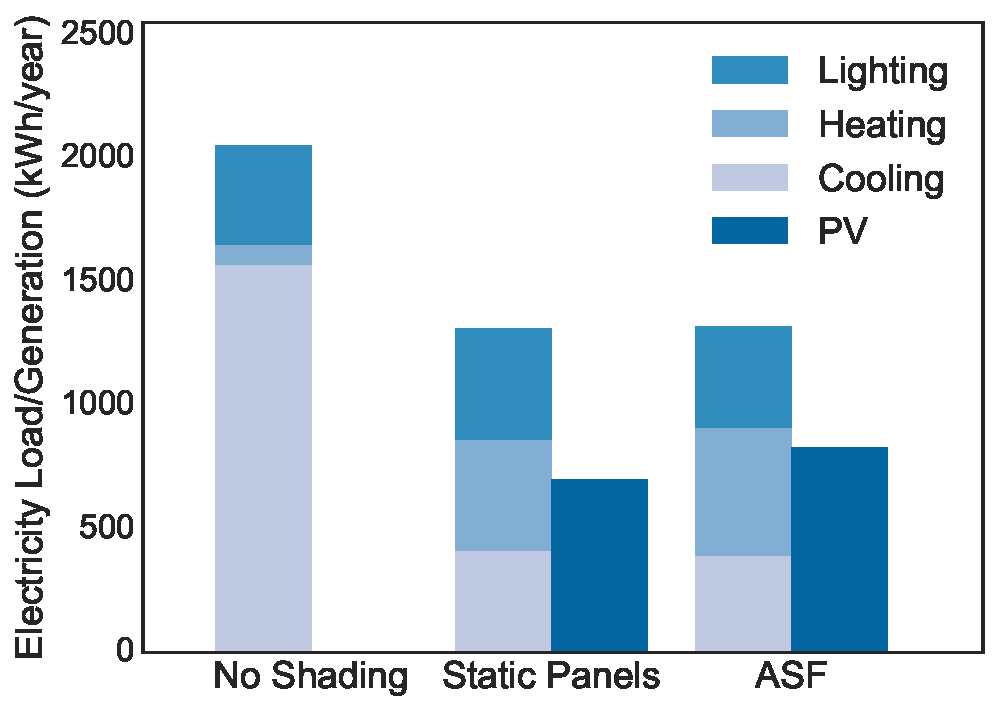
\includegraphics[width=\textwidth]{compare_facadesCOP3.pdf}
        \caption{$COP_{heating}=3$, $COP_{cooling}=3$}
        \label{fig:COP33}
    \end{subfigure}
    \hfill
    \begin{subfigure}[b]{0.47\textwidth}
        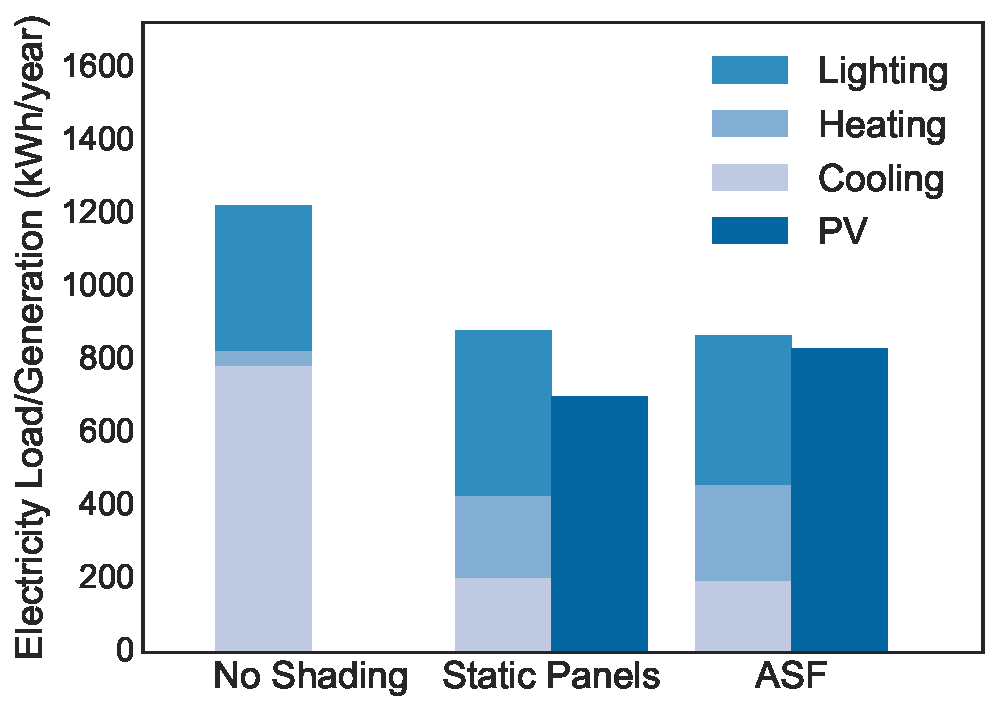
\includegraphics[width=\textwidth]{compare_facadesCOP6.pdf}
        \caption{$COP_{heating}=6$, $COP_{cooling}=6$}
        \label{fig:COP66}
    \end{subfigure}
    \caption{Breakdown of the operational electricity consumption with no shading, with static panels at 45$^{\circ}$, and an ASF for different coefficients of performance of the heating and cooling system. (a) represents an inefficient heating and cooling system, (b) represents a standard cooling system with resistive heating, (c) represents a standard heat pump system for heating and cooling, and (d) represents a high efficiency heating and cooling system.}
    \label{fig:compare}
\end{figure}

\begin{table}
\centering

\begin{tabular}{cc|cc}


$COP_{heating}$ & $COP_{cooling}$ & ASF vs No Shading & ASF vs Static  \\
                &                 & ($$kWh/year$$)    & ($$kWh/year$$) \\
\hline 
1               & 1               & 3750  (70\%)     & 724  (31\%)   \\
1               & 3               & 1370  (62\%)      & 670  (44\%)    \\
3               & 3               & 1560  (76\%)      & 120  (20\%)    \\
6               & 6               & 1190  (97\%)      & 145  (80\%)    \\

\end{tabular}
\caption{Net electricity savings of the ASF to a building with no shading, and a static photovoltaic shading system in kWh/year.}
\label{tab:compare}
\end{table}


